\documentclass[aspectratio=169]{beamer}

%% Juego de caracteres usado en el archivo fuente: UTF-8
\usepackage{ucs}
\usepackage[utf8x]{inputenc}
\uselanguage{spanish}
%Para la identación del español
\usepackage[spanish]{babel}
\usepackage{animate}
\setbeamercovered{dynamic}
\useinnertheme{rectangles}

% There are many different themes available for Beamer. A comprehensive
% list with examples is given here:
% http://deic.uab.es/~iblanes/beamer_gallery/index_by_theme.html
% You can uncomment the themes below if you would like to use a different
% one:
%\usetheme{AnnArbor}
%\usetheme{Antibes}
%\usetheme{Bergen}
%\usetheme{Berkeley}
%\usetheme{Berlin}
%\usetheme{Boadilla}
%\usetheme{boxes}
%\usetheme{CambridgeUS}
%\usetheme{Copenhagen}
%\usetheme{Darmstadt}
%\usetheme{default}
\usetheme{Frankfurt}
%\usetheme{Goettingen}
%\usetheme{Hannover}
%\usetheme{Ilmenau}
%\usetheme{JuanLesPins}
%\usetheme{Luebeck}
%\usetheme{Madrid}
%\usetheme{Malmoe}
%\usetheme{Marburg}
%\usetheme{Montpellier}
%\usetheme{PaloAlto}
%\usetheme{Pittsburgh}
%\usetheme{Rochester}
%\usetheme{Singapore}
%\usetheme{Szeged}
%\usetheme{Warsaw}

%Para la identación del español
\usepackage[spanish]{babel}

\title{AWS vs Azure}

% A subtitle is optional and this may be deleted
%\subtitle{Optional Subtitle}

\author{Jesús Rodríguez Heras\\
Carlos Llamas Jaén\\
Iván Castillo Caro\\
Sisic Dino}
% - Give the names in the same order as the appear in the paper.
% - Use the \inst{?} command only if the authors have different
%   affiliation.

%\institute[Escuela Superior de Ingeniería] % (optional, but mostly needed)
%{
%  \inst{1}%
%  Department of Computer Science\\
%  University of Somewhere
%  \and
%  \inst{2}%
%  Department of Theoretical Philosophy\\
%  University of Elsewhere}
% - Use the \inst command only if there are several affiliations.
% - Keep it simple, no one is interested in your street address.

%\date{25 de abril de 2019}
% - Either use conference name or its abbreviation.
% - Not really informative to the audience, more for people (including
%   yourself) who are reading the slides online

%\subject{Theoretical Computer Science}
% This is only inserted into the PDF information catalog. Can be left
% out. 

% If you have a file called "university-logo-filename.xxx", where xxx
% is a graphic format that can be processed by latex or pdflatex,
% resp., then you can add a logo as follows:

% pgfdeclareimage[height=0.5cm]{university-logo}{university-logo-filename}
% \logo{\pgfuseimage{university-logo}}

% Delete this, if you do not want the table of contents to pop up at
% the beginning of each subsection:
\AtBeginSection[]
{
  \begin{frame}<beamer>{Índice}
    \tableofcontents[currentsection]
  \end{frame}
}
%\AtBeginSubsection[]
%{
%	\begin{frame}<beamer>{Índice}
%	\tableofcontents[currentsection,currentsubsection]
%\end{frame}
%}

% Let's get started
\begin{document}

\begin{frame}
  \titlepage
%  \begin{center}
%  Luis Gutiérrez Flores\\
%Nicolás Ruiz Requejo\\
%Jesús Rodríguez Heras\\
%Arantzazu Otal Alberro\\
%Alejandro Segovia Gallardo\\
%Alejandro José Caraballo García\\
%Gabriel Fernando Sánchez Reina	
%  \end{center}
  
\end{frame}

\begin{frame}{Índice}
\small\tableofcontents
\end{frame}
\normalsize

\section{AWS vs Azure}
\subsection{AWS}
\begin{frame}{AWS}
	\begin{block}{What is AWS?}
		Amazon Web Services (AWS), is a collection of public cloud computing web services launched by Amazon.
	\end{block}
	\begin{block}{Features of AWS}
		\begin{itemize}
			\item Launched 13 years ago.
			\item Cloud platform, offering over 165 fully featured services from data centers globally.
			\item Largest community of customers and partners.
			\item Fastest pace of innovation.
			\item Most proven operational expertise.
			\item Only pay for what you use.
			\item Redundancy anda availability across the world.
		\end{itemize}
	\end{block}
\end{frame}

\begin{frame}{AWS}
	\begin{block}{Capacities of AWS}
		\begin{itemize}
			\item Highly durable storage: Amazon Glacier, Amazon S3, Amazon EBS
			\item Low cost computing: Amazon EC2
			\item High performance data bases: A. Redshift, A. DynamoDB, A. Elasticache, A. RDS
			\item Managing tools: A. CloudWatch, AWS IAM, AWS Cloudformation, AWS Beanstalk
		\end{itemize}
	\end{block}
\end{frame}

\begin{frame}{AWS}
	\begin{block}{Limits of AWS}
		\begin{itemize}
			\item \textbf{Amazon EC2:} Has limits on both the type of instance (virtual machine) that can be used and the number of hours in a month (750 Linux/750 Windows).
			\item \textbf {Amazon S3:} You have a limit on the amount of storage that can be used and the frequency with which you can call certain operations each month.
			\item \textbf{Amazon RDS:} You have a limit of 750 hours per month during the first 12 months. Turning on an instance three hours is the same as turning on an instance three times in one hour.
		\end{itemize}
	\end{block}
\end{frame}

\subsection{Azure}
\begin{frame}{Azure}
\begin{block}{What is Azure?}
	It is a collection of public cloud computing web services launched by Microsoft.
\end{block}
\begin{block}{Features of Azure}
	\begin{itemize}
		\item Launched in 2010.
		\item Collection of various cloud computing service.
		\item Integrated suite of tools, templates, and managed services.
		\item It provides software as a service (SaaS), platform as a service (PaaS) and infrastructure as a service (IaaS).
		\item Ideal for businesses that utilize Windows or Linux for their operations.
		\item Has over 100 services equipped with end-to-end features.
	\end{itemize}
\end{block}
\end{frame}

\begin{frame}{Azure}
\begin{block}{Capacities of Azure}
	\begin{columns}
		\column{0.5\textwidth}
		\begin{itemize}
			\item Build websites with ASP.NET, PHP or Node.js.
			\item Migrate applications and infrastructure.
			\item SQL Database.
			\item Caching.
			\item CDN.
			\item Virtual Network.
		\end{itemize}
		\column{0.45\textwidth}
		\begin{itemize}
			\item Deploy and run Windows Server and Linux virtual machines.
			\item Mobile Services.
			\item Cloud Services.
			\item Business Analytics.
			\item Hadoop.
			\item Media Services.
		\end{itemize}
	\end{columns}
\end{block}
\end{frame}

\begin{frame}{Azure}
	\begin{block}{Limits of Azure}
		In the student version, Azure has the following limits:
		\begin{itemize}
			\item 750 hours of virtual machines for both Linux and Windows.
			\item 128GB of SSD storage.
			\item 250GB of a standard S0 instance of SQL databases.
			\item 1500 hours of dynamic IP for virtual machines.
		\end{itemize}
	\end{block}
\end{frame}

\section{Comparación de los servicios ofrecidos por AWS y Azure}
\subsection{Creación de máquinas virtuales}
\subsubsection{Creación de máquinas virtuales en AWS}
\begin{frame}{Creación de máquinas virtuales en AWS}
	\begin{figure}[h]
		\centering
		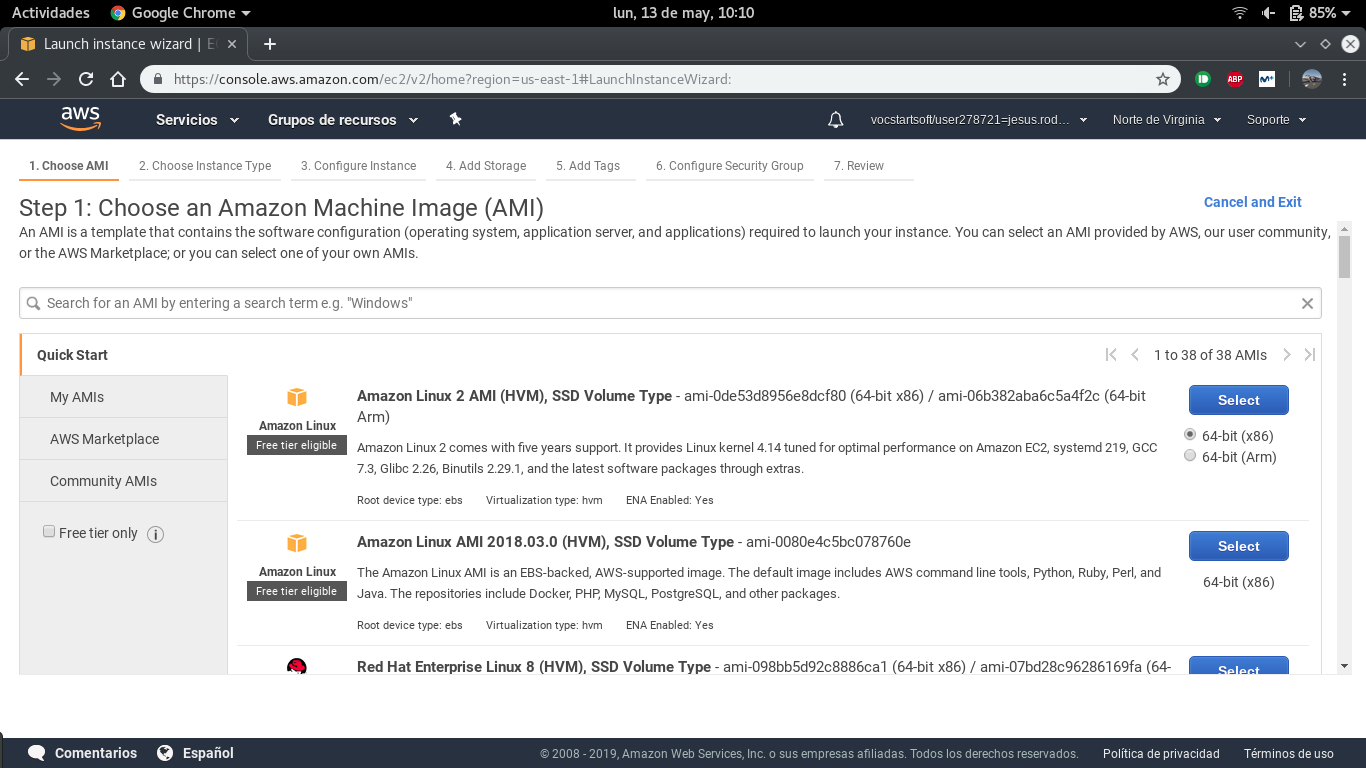
\includegraphics[scale=0.23]{AWS/MV/4.png}
		\caption{Selección de sistema operativo.}
		\label{Sistema operativo}
	\end{figure}
\end{frame}

\begin{frame}{Creación de máquinas virtuales en AWS}
\begin{figure}[h]
	\centering
	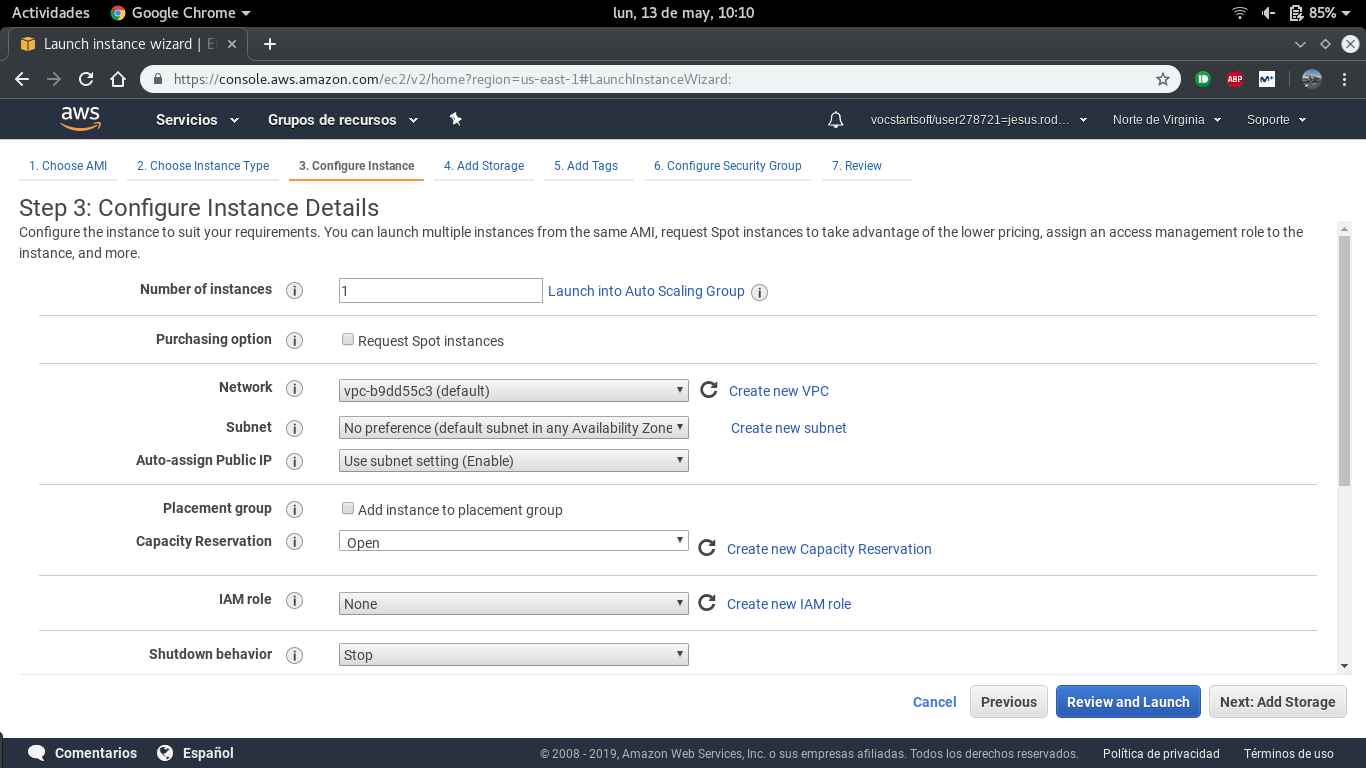
\includegraphics[scale=0.23]{AWS/MV/7.png}
	\caption{Configurar detalles.}
	\label{Configurar detalles}
\end{figure}
\end{frame}

\begin{frame}{Creación de máquinas virtuales en AWS}
\begin{figure}[h]
	\centering
	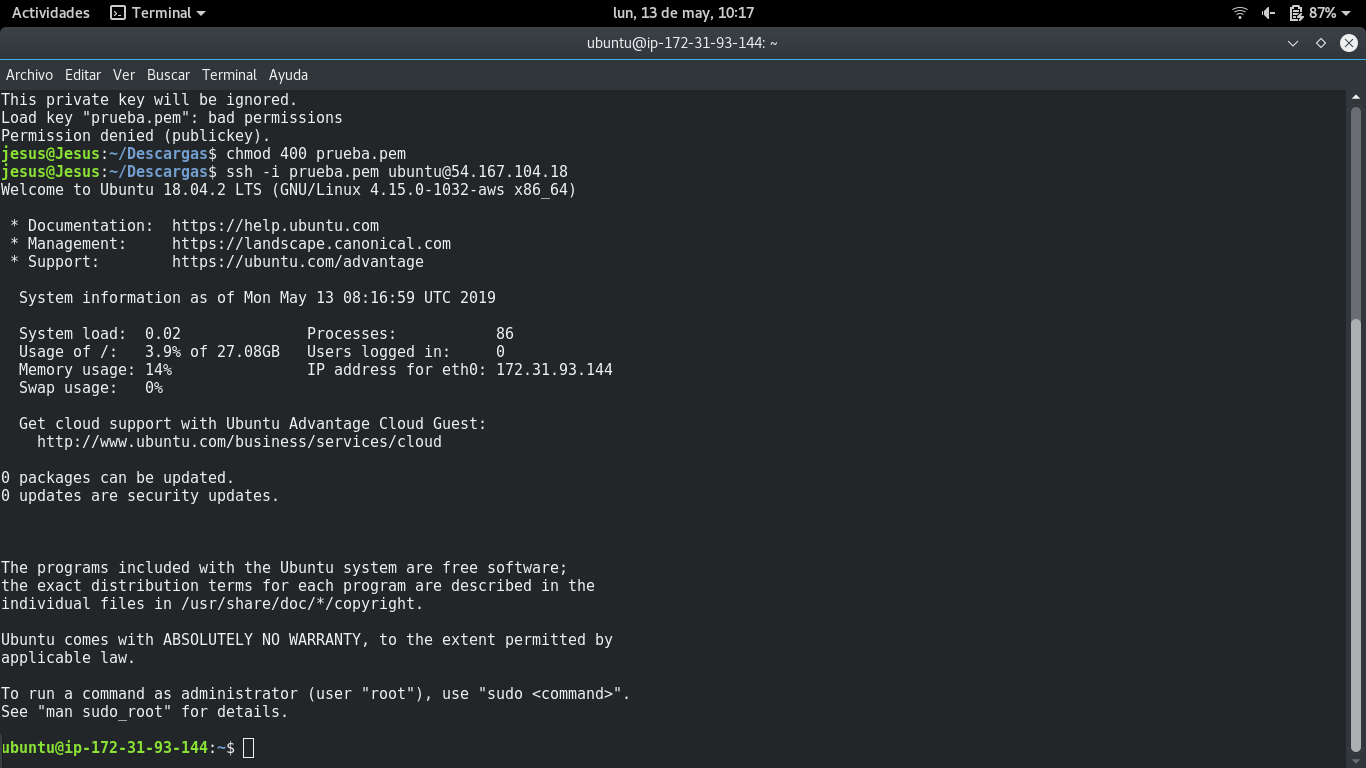
\includegraphics[scale=0.23]{AWS/MV/16.png}
	\caption{Conexión por SSH.}
	\label{SSH}
\end{figure}
\end{frame}

\subsubsection{Creación de máquinas virtuales en Azure}
\begin{frame}{Creación de máquinas virtuales en Azure}
	\begin{figure}[h]
		\centering
		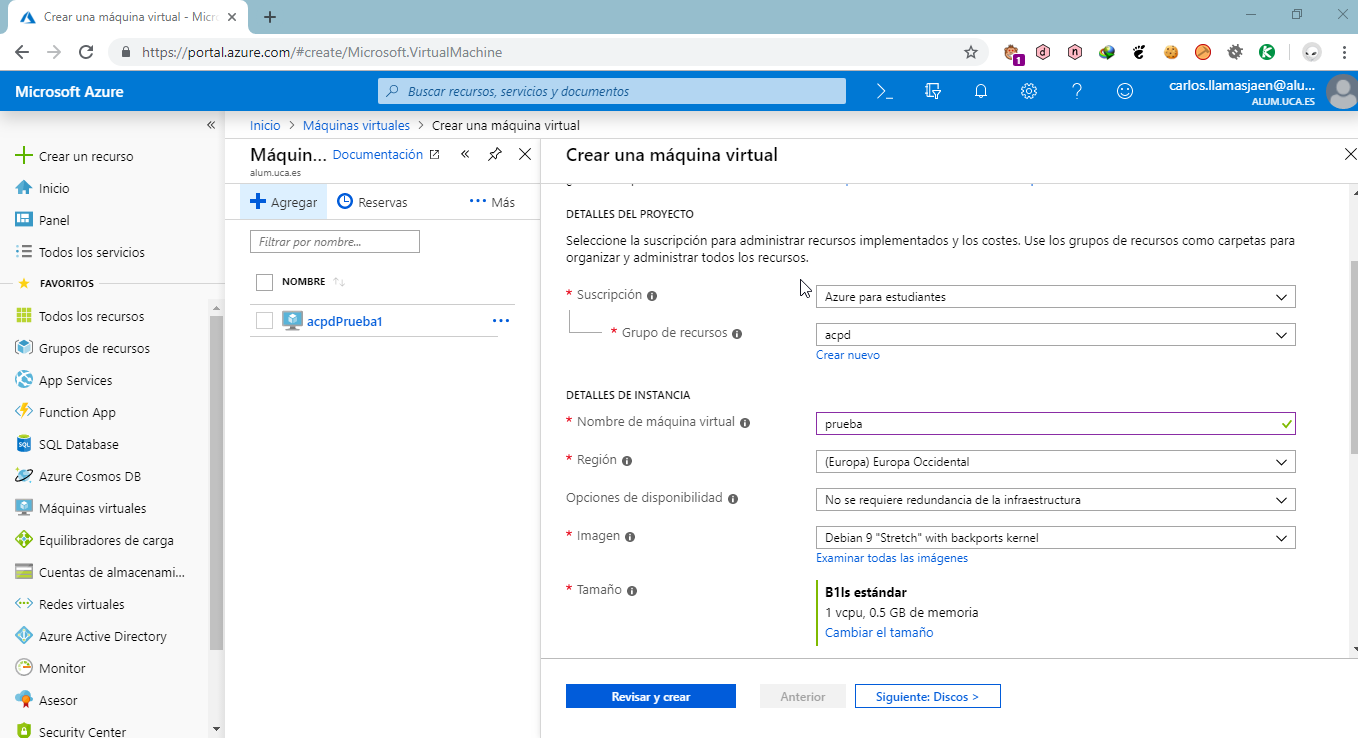
\includegraphics[scale=0.32]{Azure/MV/1.png}
		\caption{Selección de sistema operativo.}
		\label{Sistema operativo2}
	\end{figure}
\end{frame}

\begin{frame}{Creación de máquinas virtuales en Azure}
\begin{figure}[h]
	\centering
	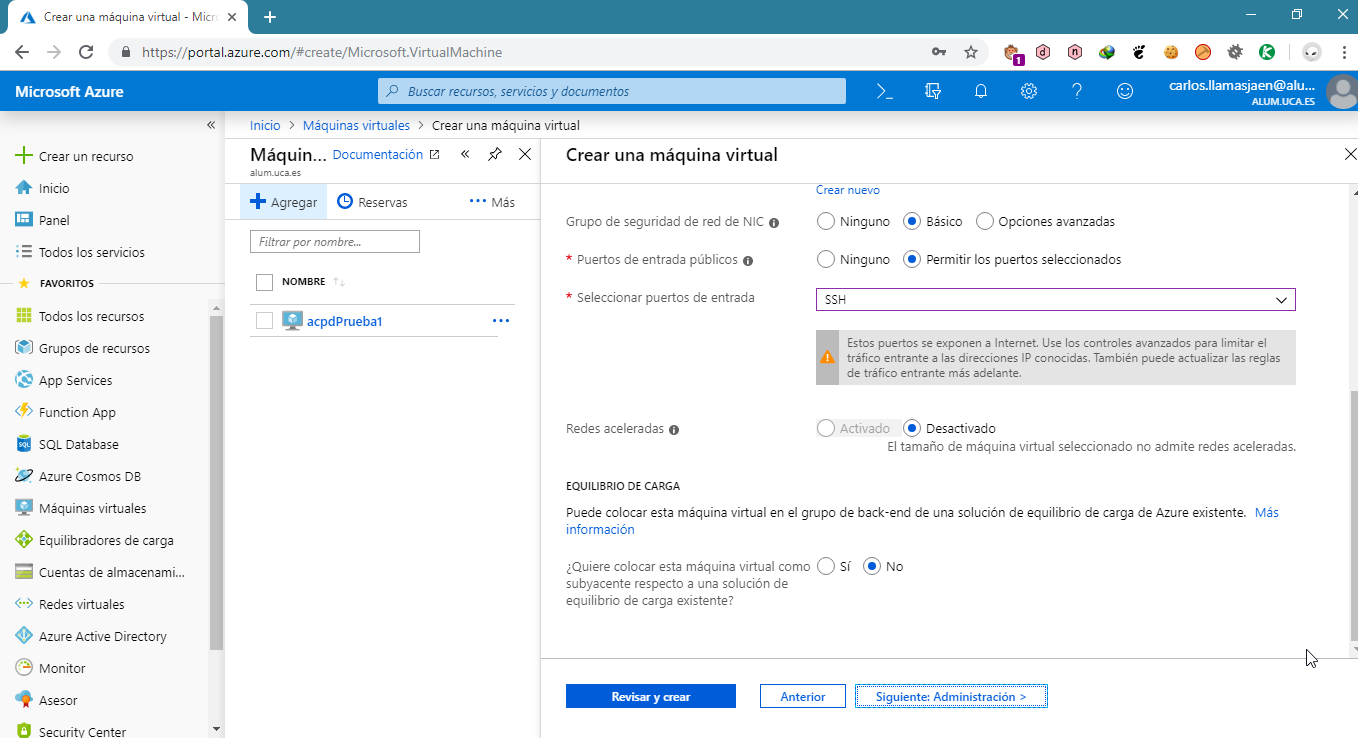
\includegraphics[scale=0.32]{Azure/MV/5.png}
	\caption{Selección como equilibrio de carga.}
	\label{Equilibrio de carga}
\end{figure}
\end{frame}

\begin{frame}{Creación de máquinas virtuales en Azure}
\begin{figure}[h]
	\centering
	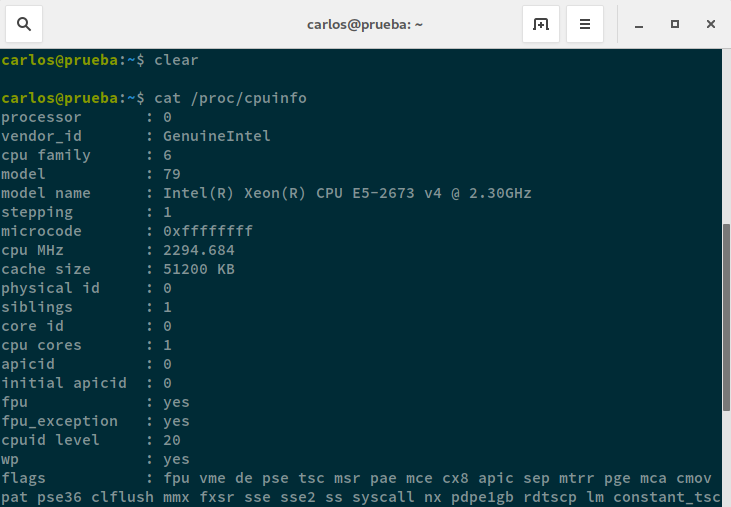
\includegraphics[scale=0.35]{Azure/MV/cpuinfo.png}
	\caption{Conexión por SSH.}
	\label{SSH2}
\end{figure}
\end{frame}

\subsection{Creación de webs}
\subsubsection{Servicios Web}
\begin{frame}{Web Services}
\begin{block}{What are web services?}
	\begin{itemize}
		\item Piece of software that makes itself available over the internet.
		\item Uses a standardized XML messaging system.
		\item Are not tied to any OS, so they work independently and concurrently.
		\item Are built on top of open standards such as TCP/IP, HTTP, Java, HTML, and XML.
	\end{itemize}
\end{block}
\begin{block}{Components}
	\begin{itemize}
		\item SOAP (Simple Objet Protocol).
		\item UDDI (Universal Description, Discovery and Integration).
		\item WSDL (Web Services Description Language).
	\end{itemize}
\end{block}
\end{frame}

\subsubsection{Creación de webs en AWS}
\begin{frame}{Creación de webs en AWS}
	\begin{figure}[h]
		\centering
		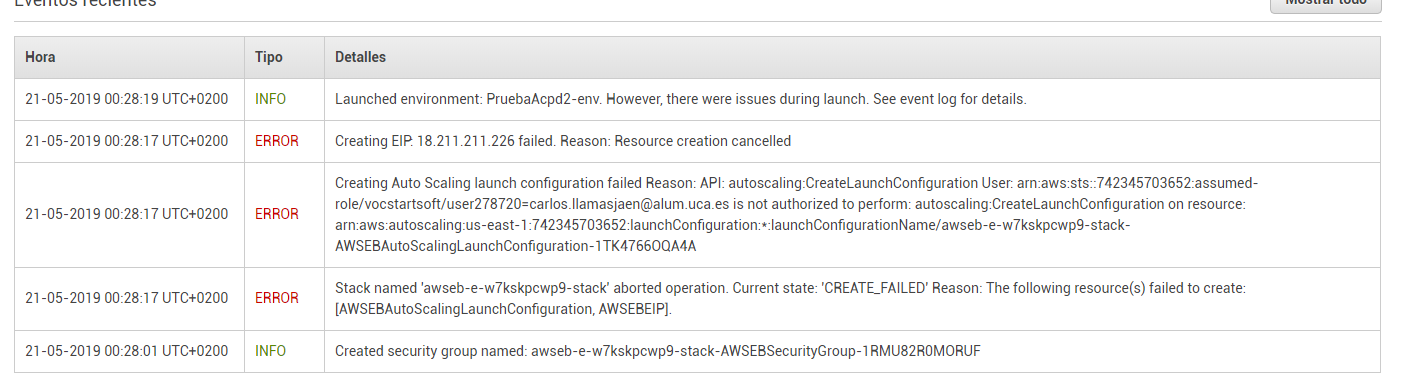
\includegraphics[scale=0.39]{AWS/Web/error_aws.png}
		\caption{Error en la creación de aplicación web de AWS.}
		\label{Error AWS}
	\end{figure}
\end{frame}

\subsubsection{Creación de webs en Azure}
\begin{frame}{Creación de webs en Azure}
	\begin{figure}[h]
		\centering
		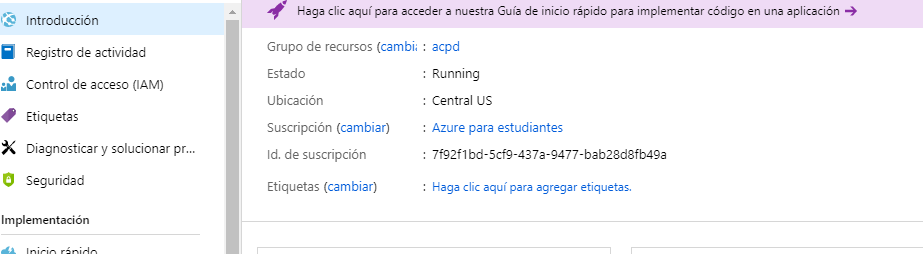
\includegraphics[scale=0.55]{web_azure/centro.png}
		\caption{Centro de aplicaciones web de Azure.}
		\label{Centro de aplicaciones web de Azure}
	\end{figure}
\end{frame}

\begin{frame}{Creación de webs en Azure}
\begin{figure}[h]
	\centering
	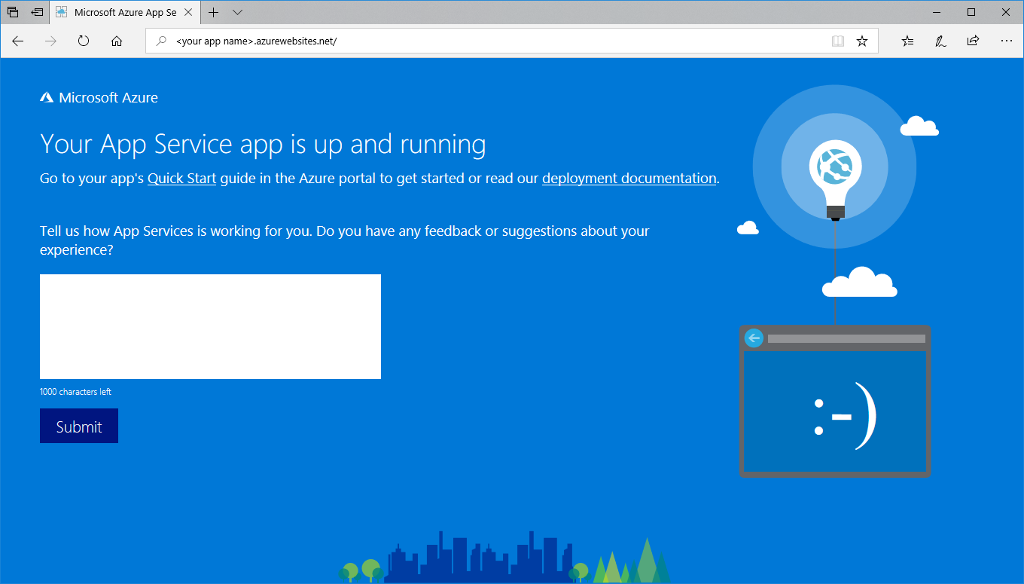
\includegraphics[scale=0.3]{web_azure/web1.png}
	\caption{Ejemplo de web.}
	\label{Ejemplo de web}
\end{figure}
\end{frame}

\subsection{Creación de servicios IoT}
\subsubsection{Creación de servicios IoT en AWS}
\begin{frame}{Creación de servicios IoT en AWS}
	\begin{figure}[h]
		\centering
		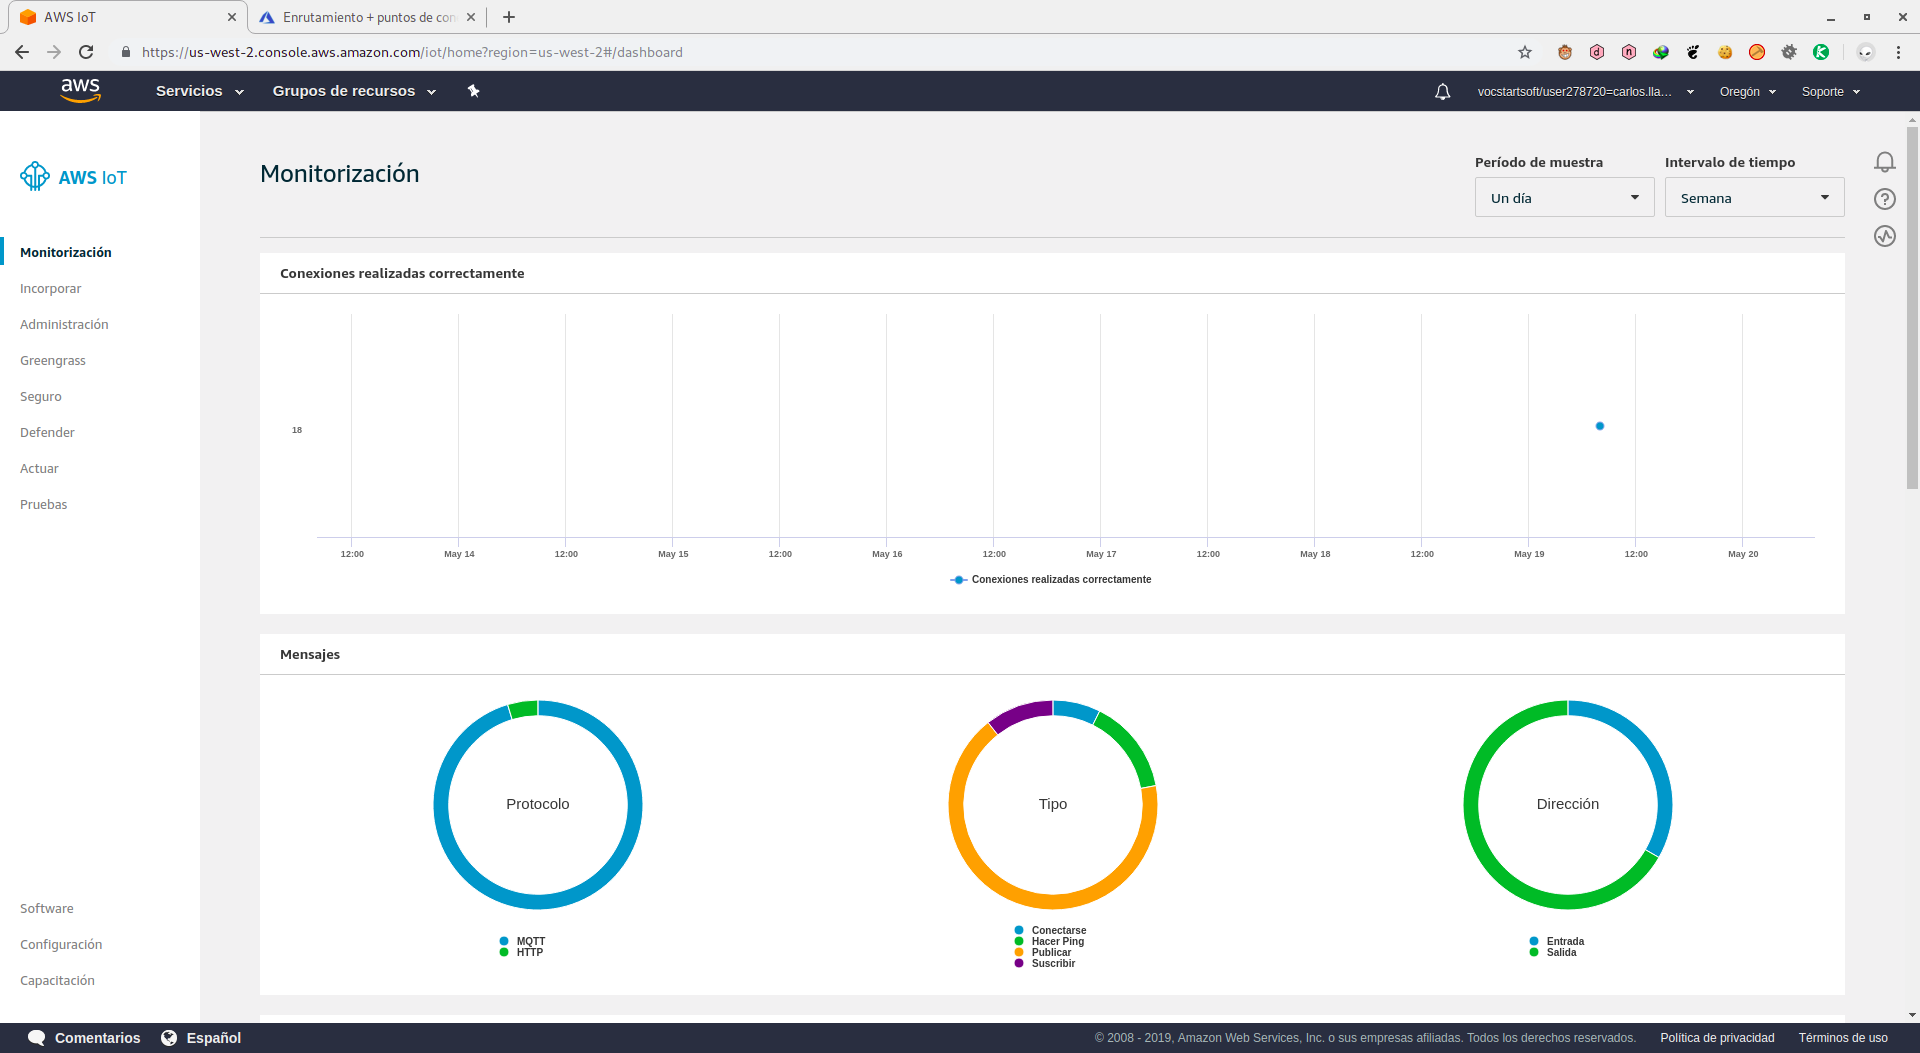
\includegraphics[scale=0.17]{iot_aws/centro.png}
		\caption{Centro de control de IoT de AWS.}
		\label{Centro de control de IoT de AWS}
	\end{figure}
\end{frame}

\begin{frame}{Creación de servicios IoT en AWS}
\begin{figure}[h]
	\centering
	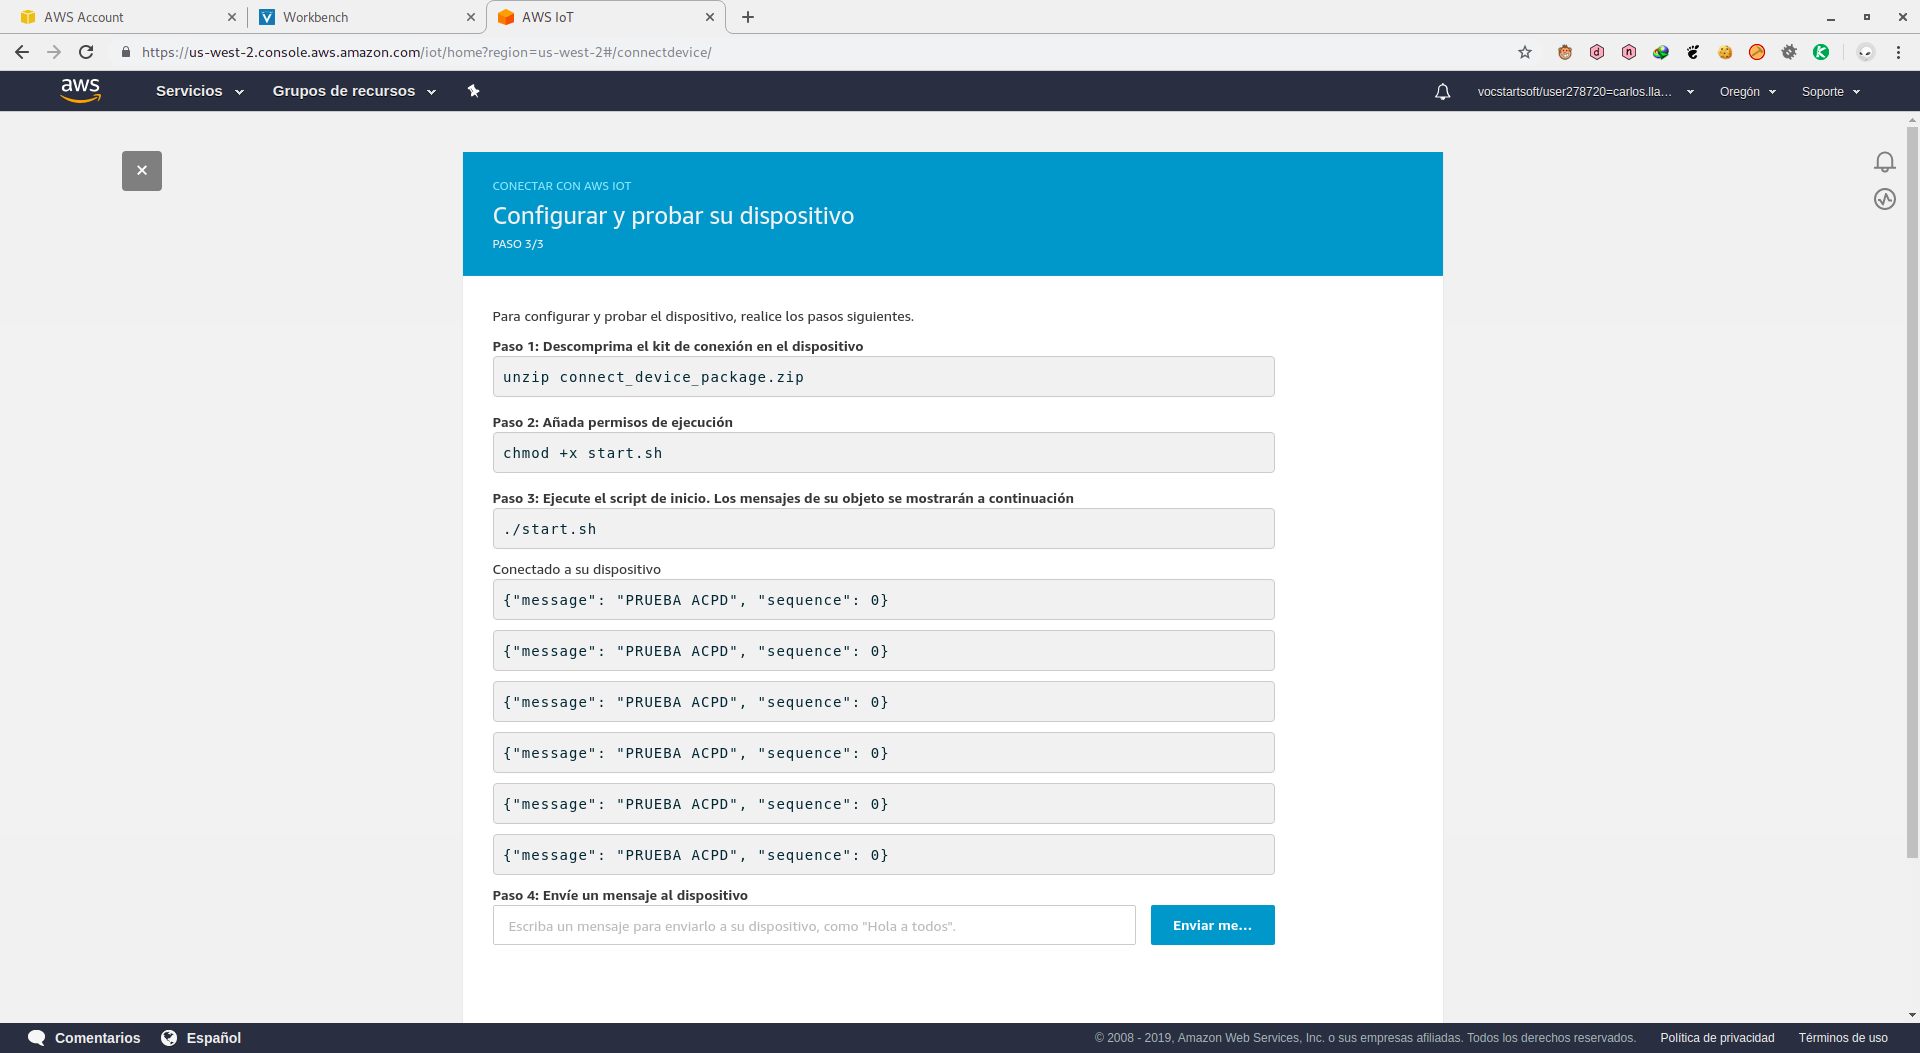
\includegraphics[scale=0.17]{iot_aws/creacion5.png}
	\caption{Dispositivos IoT de AWS.}
	\label{Dispositivo IoT de AWS}
\end{figure}
\end{frame}

\subsubsection{Creación de servicios IoT en Azure}
\begin{frame}{Creación de servicios IoT en Azure}
\begin{figure}[h]
	\centering
	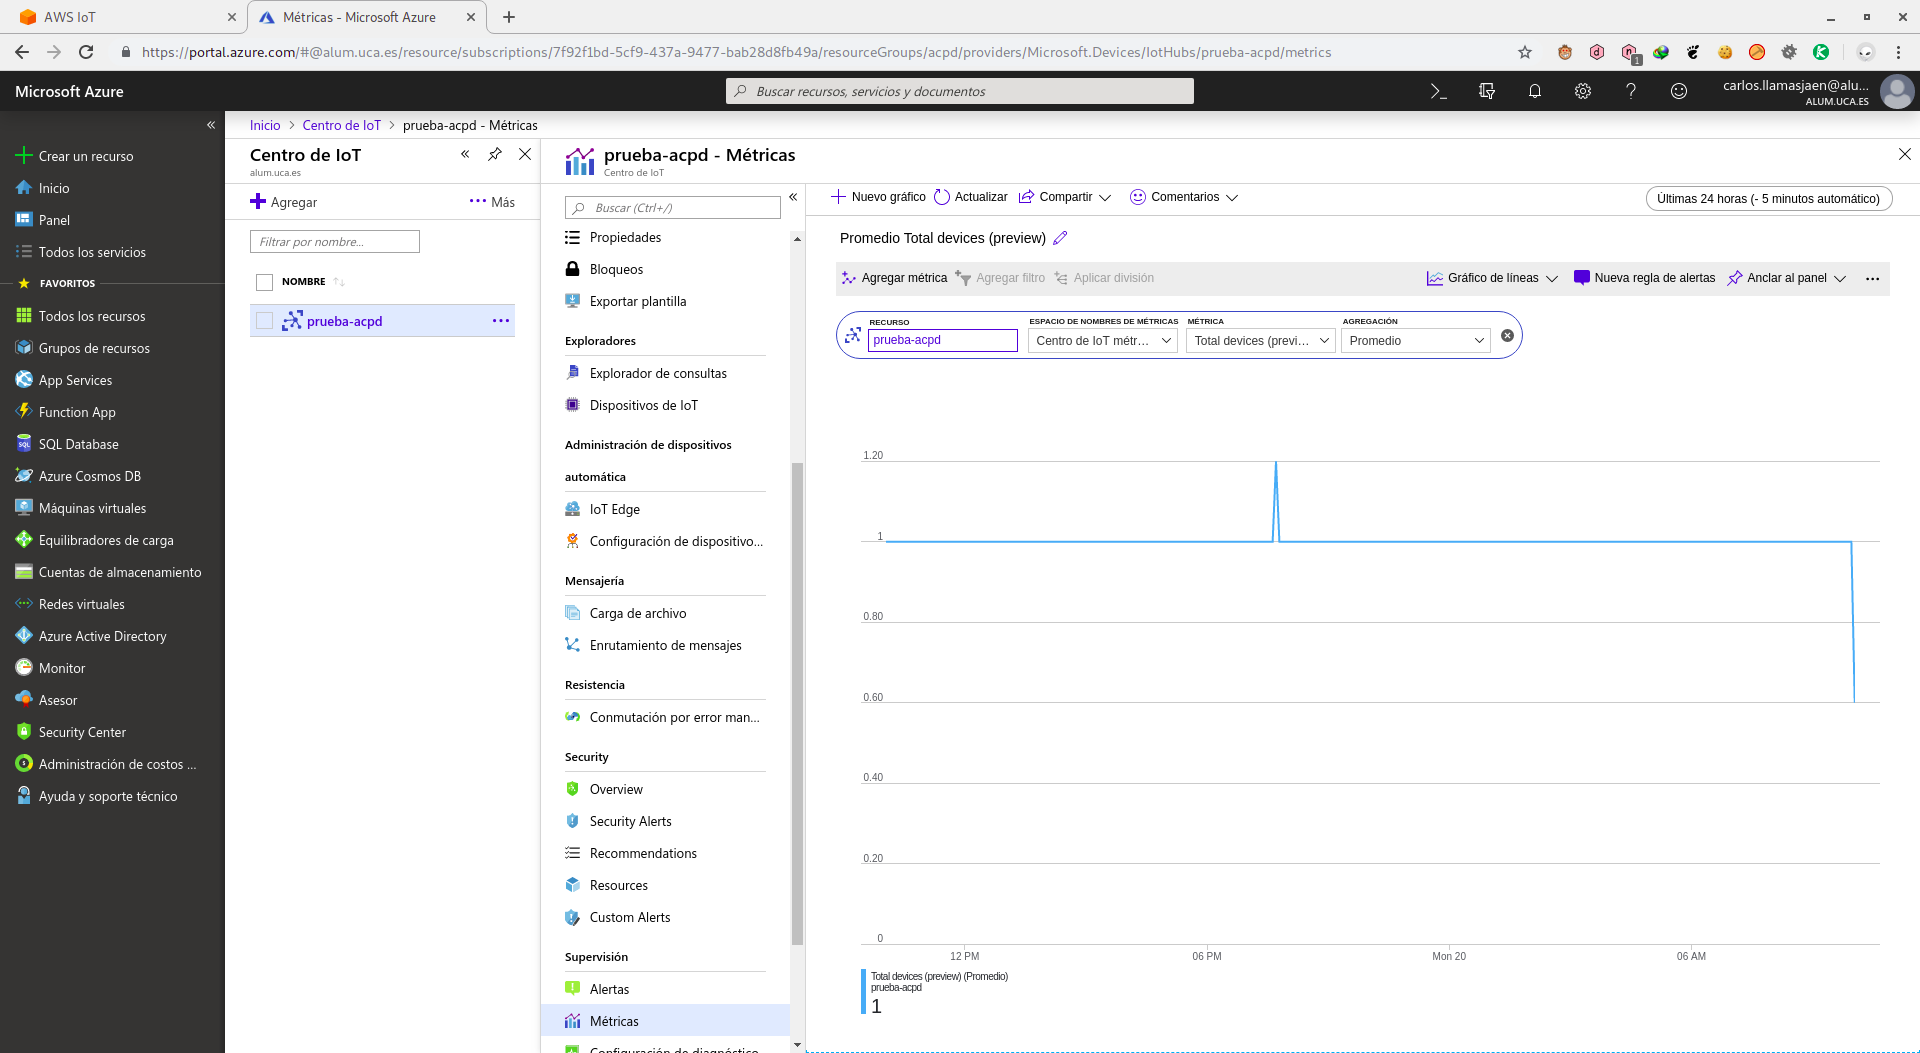
\includegraphics[scale=0.17]{iot_azure/centro2.png}
	\caption{Centro de control de IoT de Azure.}
	\label{Centro de control de IoT de Azure}
\end{figure}
\end{frame}

\begin{frame}{Creación de servicios IoT en Azure}
\begin{figure}[h]
	\centering
	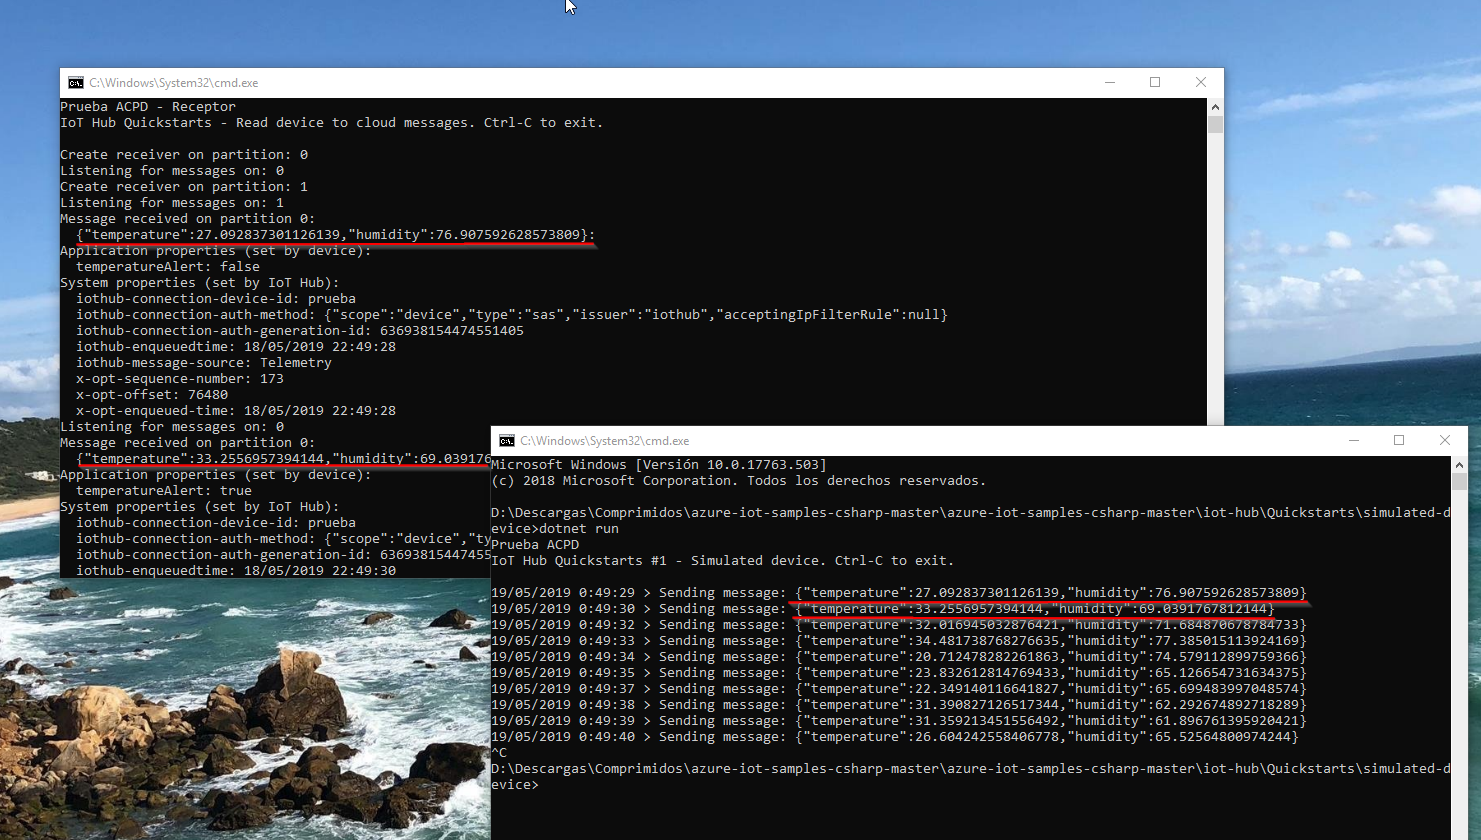
\includegraphics[scale=0.285]{iot_azure/mensajes.png}
	\caption{Dispositivo de IoT de Azure.}
	\label{Dispositivo de IoT de Azure}
\end{figure}
\end{frame}


\end{document}


